\documentclass{beamer}
\usepackage[utf8]{inputenc}
\usetheme{default}
\title{Low Extra Delay Background Transport (LEDBAT)}
\author{Arseny Kurnikov\\
Harri Hämäläinen}
\begin{document}


\begin{frame}
\titlepage
\end{frame}

\begin{frame}{Low Extra Delay Background Transport (LEDBAT)}
    \begin{itemize}
        \item A delay based congestion control algorithm
        \item Lower-than-best-effort service
            \begin{itemize}
                \item Will yield to high-load flows
                \item No more aggressive than TCP
            \end{itemize}
        \item Designed especially for background bulk-transfer applications(e.g. BitTorrent)
    \end{itemize}
\end{frame}

\begin{frame}{Delay based congestion control 1}
    \begin{itemize}
        \item One-way delay measurement
        \item Delay is seen as a sum of:
            \begin{itemize}
                \item Base delay: the minimum observed delay on the end-to-end
                path within a specified window
                \item Queuing delay: the difference of the base delay and the
                current estimate of base delay
            \end{itemize}
        \item The delays are computed as an average over a sliding window and outliers are
        filtered to obtain steady values
        \item The congestion window is also controlled by the delay based linear
        controller of LEDBAT in addition to traditional TCP controls
    \end{itemize}
\end{frame}

\begin{frame}{Delay based congestion control 2}
    \begin{itemize}
        \item When the queuing delay is smaller than the target delay the
        congestion window is increased proportionally to the relative difference
        of queuing and target delays
        \begin{itemize}
            \item As the queuing delay gets closer to the target delay the
            growth of congestion window size slows down
            \item The highest rate of window growth is as it is with TCP (when
            queuing delay estimate is zero)
        \end{itemize}

        \item When the queuing delay is higher than the target delay the linear
        controller of LEDBAT allows the congestion window to be decreased
        proportionally to the difference of queuing and target delays.
        \begin{itemize}
            \item No packet losses are required for the congestion window to be
            decreased
            \item If a packet loss however occurs the response to this event
            must be as it is with TCP
        \end{itemize}
    \end{itemize}
\end{frame}

\begin{frame}{Fairness}
    \begin{itemize}
        \item LEDBAT yields to high-load flows
        \item In any case it is no more aggressive than TCP
        \item Currently fairness among LEDBAT flows cannot be guaranteed in all cases
            \begin{itemize}
                \item Latecomers can incorrectly measure a base delay on
                bottleneck link saturated by another LEDBAT flow
                \item In practice we usually recover from this scenario due to
                caps in transmission allowing the latecomer to measure the base
                delay correctly
            \end{itemize}
    \end{itemize}
\end{frame}

\begin{frame}{Throughput of competing flows}
    \begin{columns}
    \begin{column}[l]{5cm}
        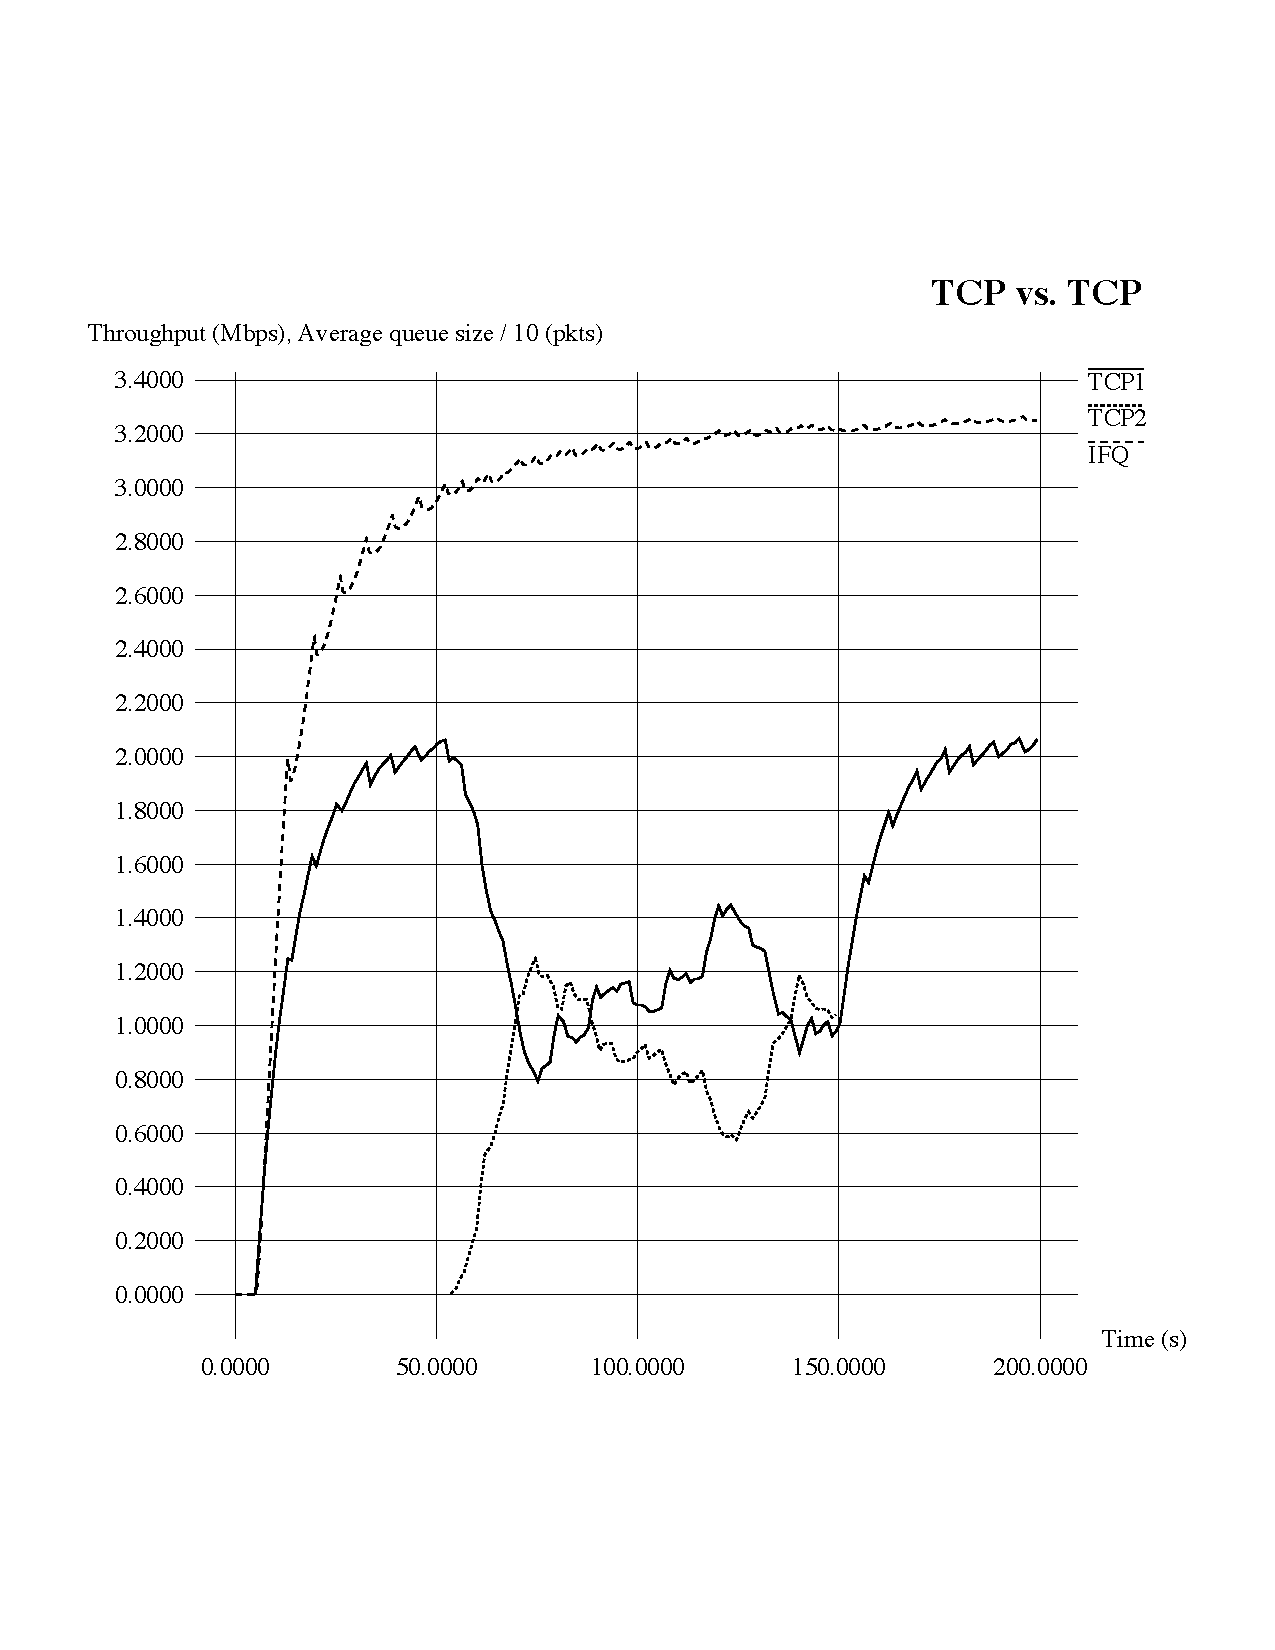
\includegraphics[scale=0.25]{tcp.pdf}
    \end{column}
    \begin{column}[r]{5cm}
        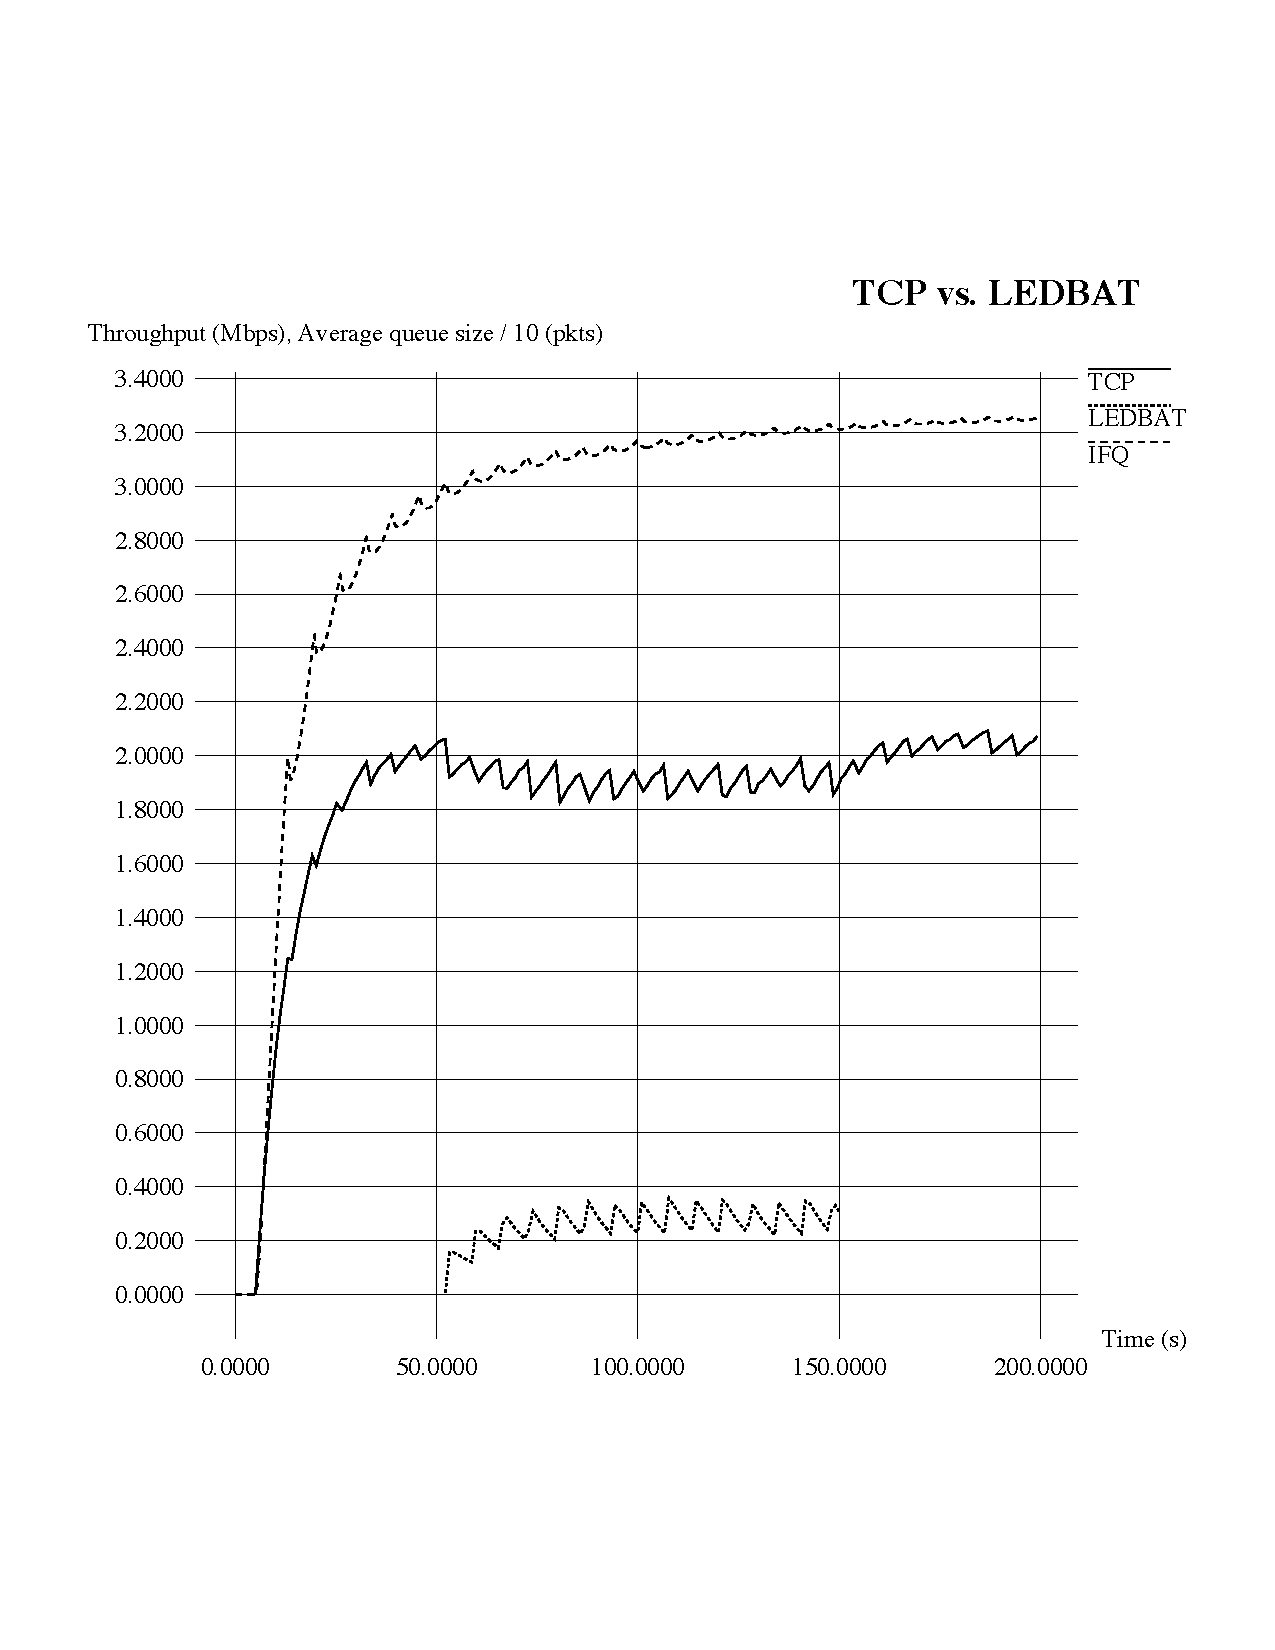
\includegraphics[scale=0.25]{tcpledbat.pdf}
    \end{column}
    \end{columns}
\end{frame}

\begin{frame}{Sources}
    \begin{itemize}
        \item RFC6817, \url{http://tools.ietf.org/html/rfc6817}
        \item Dario Rossi :: Software / LEDBAT,
        \url{http://perso.telecom-paristech.fr/~drossi/index.php?n=Software.LEDBAT}
    \end{itemize}
\end{frame}

\end{document}
